
\textbf{Project name :}QTypingTest \\
\textbf{Project Supervisor :} Marc Cummins \\
\textbf{Project start date : } 6/10/2015
\textbf{Project end date : }1/05/2016 \\
\textbf{Project Budget :} 0.00€ \\

\chapter{Objectives}
The aim of this project is to create a software capable to teach to everyone how to type faster.
The purpose of this guide will be for education and enjoyment.\\
The software will have options to choose the level of the tests. Thanks to this level system, people who do not know how to type will be able to learn, and people who already knows basics will be capable of improving their current speed.\\
The users learning from scratch will be guided from the baseline of the keyboard until the numbers at the second upper-line of the keyboard.\\
The software will be an open-source (under LGPL licence) Qt project. It will be available for the three most-used platform : 
\begin{itemize}
	\item Windows
	\item MacOs
	\item Linux
\end{itemize}
 It will be translated in differents
languages (mostly languages from Europeans country) so that no matter your native language, you can learn how to type faster.\\
All tasks will be completed by 1/05/2016.

\chapter{Activity list}
\begin{enumerate}
	\item[]\textbf{Learn how to use properly the tools}
	\item Learn how to code in C++ properly by reading a document called "CppCoreGuidelines"
	\item Learn how to use Qt 
	\begin{enumerate}
		\item Follow simple tutorial
		\item Create a simple software as example
	\end{enumerate} 
	\item Learn how to code using Qt properly
	\item[]\textbf{Implement the software}
	\item Implement the basic typing test
	\item Implement the general user interface
	\item Implement the text-copying exercise
	\item Create the database to store the users
	\item Implement the connection system
	\item Implement the score saving system
	\item Implement the differents options
	\item Create a main documentation for the project
	\item Create the translatable file
	\item Translate in differents languages (these languages will be also chosen at this moment)
	\item[]\textbf{Last steps before the release}
	\item Beta testing. Ask to people to test the software and ask them to tell us how to improve the software
	\item Last improvements
	\item Final release of the software
	\item Maintain the software
\end{enumerate}

%Gantt
\chapter{Gantt diagram}
\begin{center}
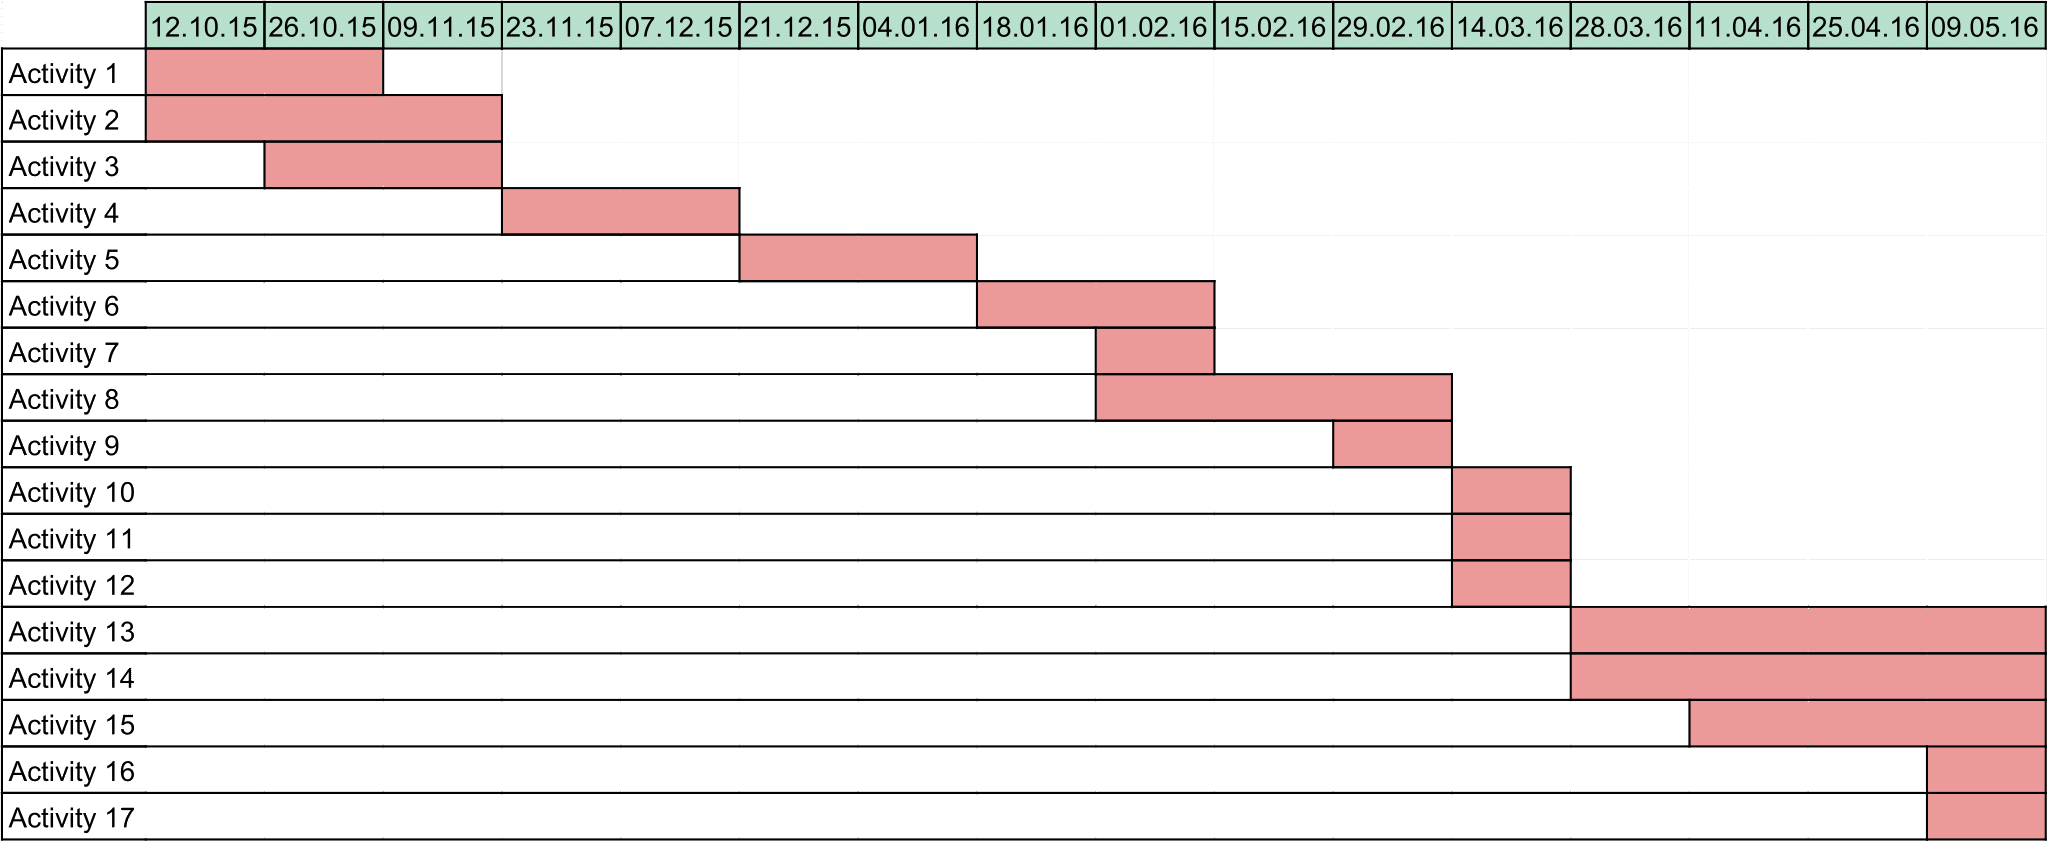
\includegraphics[scale=0.23]{./images/Gantt.png}
\end{center}


\chapter{Defining features and benefits of the software}
The benefits of this product are that it will teach the user how to type faster. The typing speed is really important today, where every company has computers and so keyboards. Not only secretary should type faster, everyone who type faster is more efficient at his work and can satisfy his responsible and/or client. The software will be free, so accessible to everyone who wants to use it. \\
Not only english, but a lots of others languages will be available in the software. So if you want to improve your typing speed in your native language you can. Moreover you can improve your speed in others languages.
Another advantage of this software licence. Furthermore, people who wants to improve the software are free to do it as it is an open source project. 
